\documentclass[letterpaper,12pt]{article}
\usepackage[utf8]{inputenc}
\usepackage[spanish]{babel}
\usepackage{tabularx} % extra features for tabular environment
\usepackage{amsmath}  % improve math presentation
\usepackage{graphicx} % takes care of graphic including machinery
\usepackage[margin=1in,letterpaper]{geometry} % decreases margins
\usepackage{cite} % takes care of citations
\usepackage[final]{hyperref} % adds hyper links inside the generated pdf file
\hypersetup{
	colorlinks=true,       % false: boxed links; true: colored links
	linkcolor=blue,        % color of internal links
	citecolor=blue,        % color of links to bibliography
	filecolor=magenta,     % color of file links
	urlcolor=blue         
}
\usepackage{blindtext}
%++++++++++++++++++++++++++++++++++++++++


\begin{document}

\title{Introducción a la Mecánica Teórica: Tarea 1}
\author{Carlos Manuel Rodríguez Martínez}
\date{\today}
\maketitle

\begin{abstract}
Tarea de aplicación del principio de D´Alembert y ecuaciones de Euler-Lagrange
\end{abstract}


\section{Introducción}

El principio de D'Alembert y el formalismo Lagrangiano nos permiten expresar y obtener las ecuaciones de movimiento de un sistema dinámico a través de un formalismo diferente al de Newton. El objetivo de esta tarea es que los estudiantes exploren el planteamiento de soluciones a partir de estos formalismos de manera que puedan apreciar cómo se diferencían del formalismo Newtoniano.


\section{Principio de D'Alembert}
Resolver los siguientes problemas usando el principio de D'Alembert.

\subsection{1- Máquina de Atwood}
Consideremos dos masas $m_1$ y $m_2$ unidas por un hilo que pasa por una polea ideal (sin masa y sin rozamiento) tal como se muestra en la figura \ref{fig:atwood}, de forma que ambas cuelgan verticalmente. ¿Cuál es el valor de la aceleración con la que se mueven las masas?

\begin{figure}[h!]
    \centering
    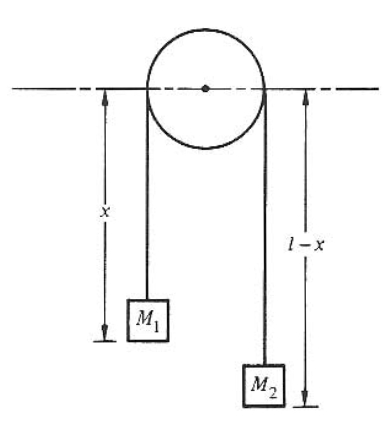
\includegraphics[width=.2\textwidth]{Atwood.png}
    \caption{Diagrama de la máquina de Atwood}
    \label{fig:atwood}
\end{figure}

Hint: Las coordenadas están relacionadas por la constricción $x_1 + x_2 = l$ que se puede expresar como $f(x_1, x_2) = x_1 + x_2 - l = 0$. El diferencial de $f$ está dado por:
\[
    \mathrm{d} f = \nabla f \cdot \mathrm{d} \vec{r} = \frac{\partial f}{\partial x} \mathrm{d}x + \frac{\partial f}{\partial y} \mathrm{d}y = 0.
\]

A partir de esta expresión podemos obtener la variación de $f$ en términos de la variación de sus coordenadas:
\[
    \delta f = \nabla f \cdot \delta \vec{r} = \frac{\partial f}{\partial x} \delta x + \frac{\partial f}{\partial y} \delta y = 0,
\]
así que en este problema tenemos que
\[
     \delta f = \delta x + \delta y = 0
\]

\subsection{2- Plano inclinado}
Consideremos ahora el caso de una partícula que desciende sin rozamiento por un plano inclinado de base $b$ y altura $h$. ¿Cuál es el valor de su aceleración?

\subsection{3- Péndulo simple cartesiano}
Consideremos el caso de un péndulo simple en el que una masa $m$ pende de un punto fijo a través de un hilo ideal de longitud $L$. La única fuerza aplicada sobre la masa es el peso, que actúa en la dirección vertical. Obtener las ecuaciones de movimiento en el sistema de coordenadas cartesianas.

Hint: Podemos expresar la constricción por medio de la función $f(x, y) = x^2 + y^2 - L^2 = 0$, comience por calcular la variación $\delta f$.

\subsection{4- Péndulo simple parametrizado}
Resuelva el mismo problema del péndulo simple pero esta vez parametrice el vector $\vec{r}(x, y)$ en términos del ángulo, esto es $\vec{r}(\theta)$.

\section{Ecuaciones de Euler-Lagrange}
Resolver los problemas 1, 2 y 3 de la sección anterior utilizando el formalismo Lagrangiano.

\end{document}
